\documentclass[border=10pt]{standalone}

\usepackage{tikz}
\usepackage{tikzsymbols}
\usetikzlibrary{calc,patterns,shapes.geometric}

\def\centerarc[#1](#2)(#3:#4:#5){\draw[#1] ($(#2)+({#5*cos(#3)},{#5*sin(#3)})$) arc (#3:#4:#5);}

\begin{document}
	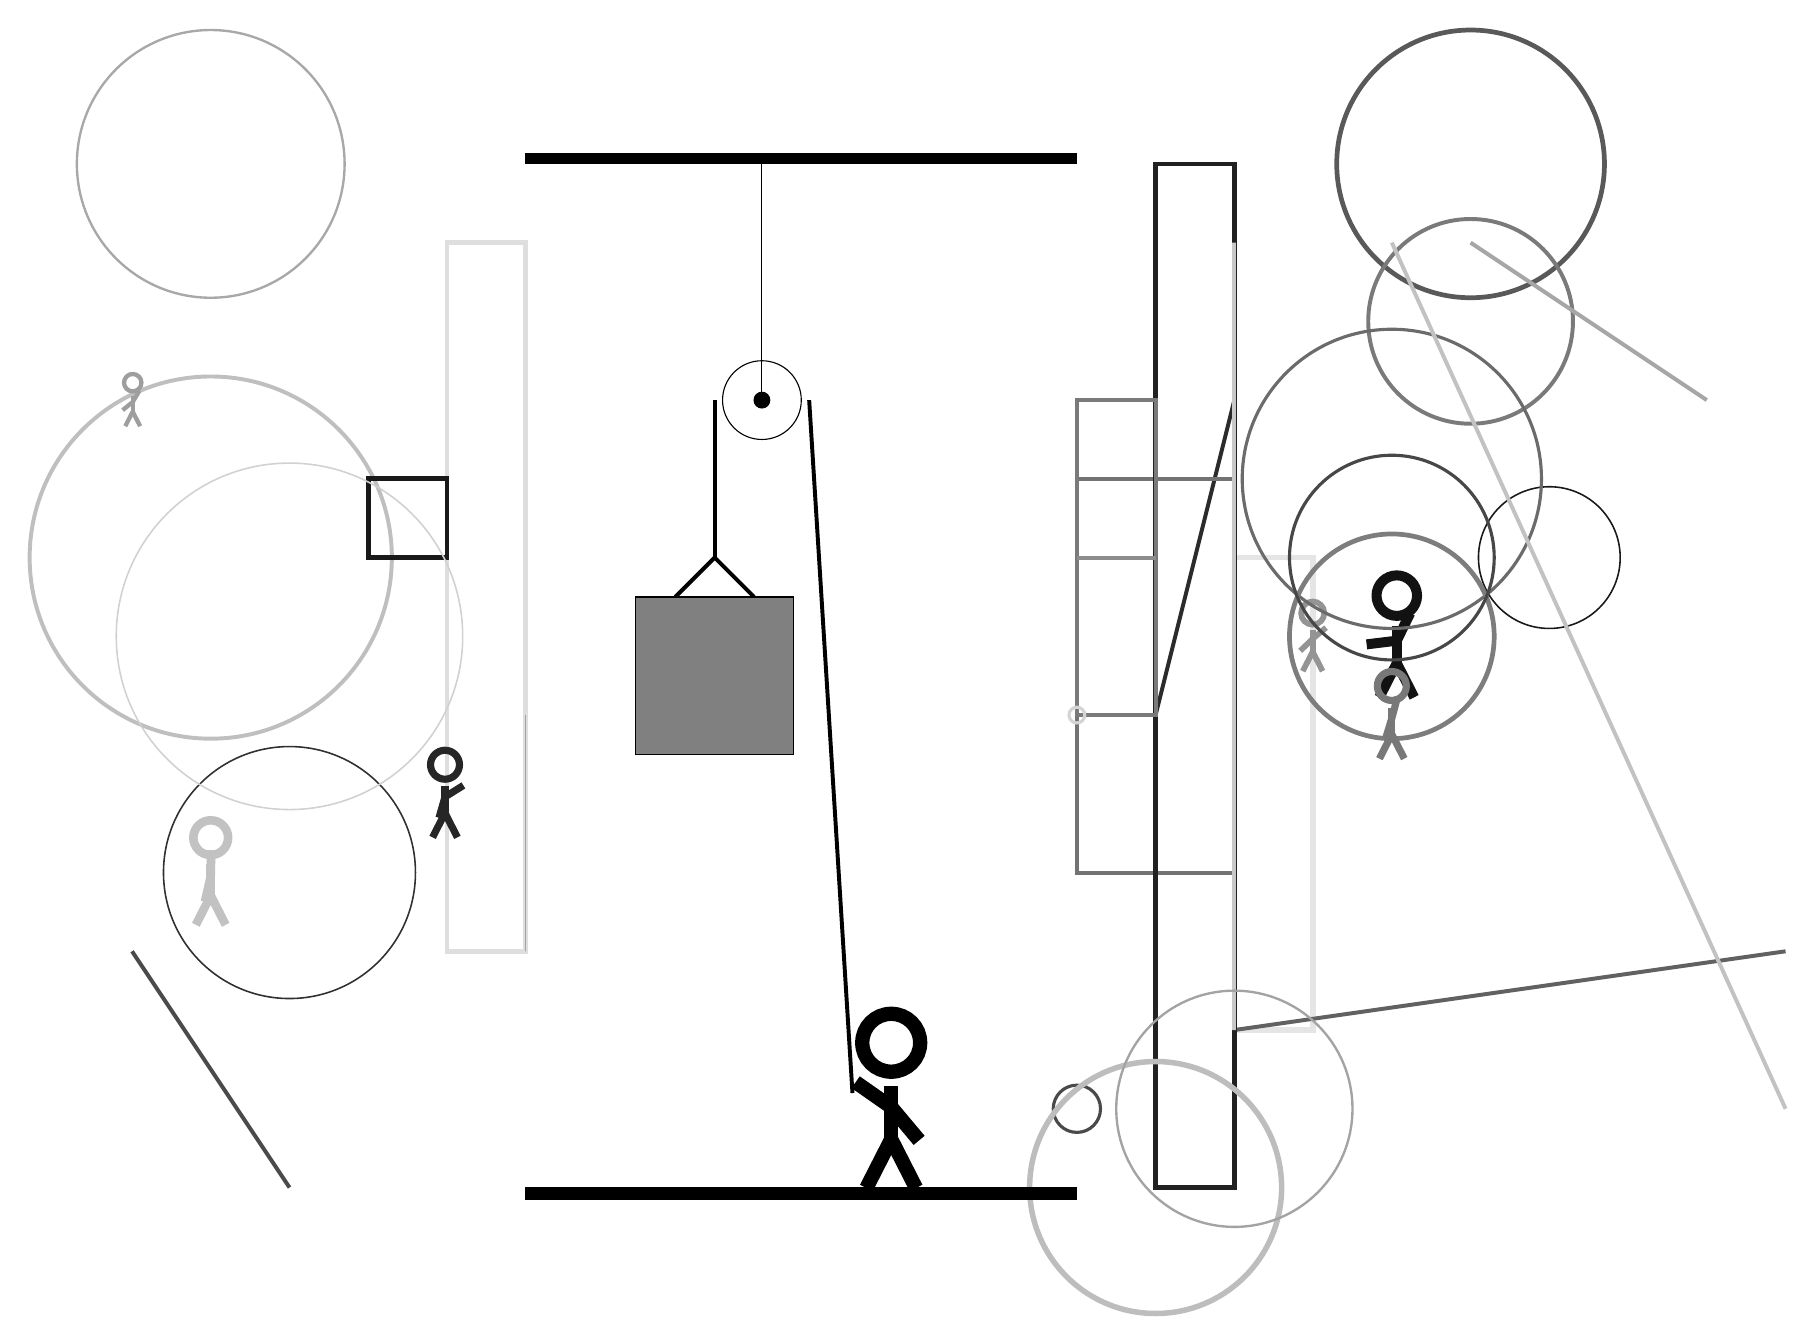
\begin{tikzpicture}
		%%%%% START %%%%%
		
		\draw[fill=black] (-2, 10) rectangle (5, 10.125);
		
		\draw (1, 7) circle (0.5);
		\draw[fill=black] (1, 7) circle (0.1);
		\draw (1, 10) -- (1, 7);
		
		\draw[line width=0.5mm] (-0.1, 4.5) -- (0.4, 5.0) -- (0.9, 4.5);
		\draw[fill=black!50] (-0.6, 4.5) rectangle (1.4, 2.5);
		
		\draw[line width=0.5mm] (0.4, 7) -- (0.4, 5.0);
		\centerarc[line width=0.5mm](1, 7)(0:180:0.6);
		\draw[line width=0.5mm](1.6, 7) -- (2.15, -1.8);
		
		\node at (2.6, -1.9) {\Strichmaxerl[10][-35][-50]};
		
		\node[line width=0.2mm, color=black!93] at (9, 4) {\Strichmaxerl[7][7][64]};
		
		\draw[line width=0.7mm, color=black!10] (7, 5) rectangle (8, -1);
		\draw[line width=0.5mm, color=black!83](7, 7) -- (6, 3);
		\draw [line width=0.2mm, color=black!90](11, 5) circle (0.9);
		\draw [line width=0.5mm, color=black!25](-6, 5) circle (2.3);
		
		\draw [line width=0.6mm, color=black!65](10, 10) circle (1.7);
		
		\draw[line width=0.5mm, color=black!62](7, -1) -- (14, 0);
		\draw[line width=0.7mm, color=black!28] (6, -3) rectangle (6, 8);
		\draw[line width=0.5mm, color=black!55] (7, 1) rectangle (5, 6);
		\draw [line width=0.5mm, color=black!52](10, 8) circle (1.3);
		\draw[line width=0.6mm, color=black!13] (-2, 0) rectangle (-3, 9);
		\node[line width=0.5mm, color=black!42] at (8, 4) {\Strichmaxerl[4][44][40]};
		\draw[line width=0.6mm, color=black!87] (7, -3) rectangle (6, 10);
		\draw[line width=0.6mm, color=black!90] (-4, 5) rectangle (-3, 6);
		\draw[line width=0.5mm, color=black!52] (6, 7) rectangle (5, 3);
		\draw [line width=0.4mm, color=black!58](9, 6) circle (1.9);
		
		\draw [line width=0.6mm, color=black!51](9, 4) circle (1.3);
		\draw [line width=0.3mm, color=black!34](-6, 10) circle (1.7);
		\draw[line width=0.5mm, color=black!21] (7, 9) rectangle (7, -1);
		\draw[line width=0.2mm, color=black!36] (-2, 3) rectangle (-2, 0);
		\node[line width=0.5mm, color=black!24] at (-6, 1) {\Strichmaxerl[6][77][89]};
		
		\draw[line width=0.5mm, color=black!24](9, 9) -- (14, -2);
		\node[line width=0.4mm, color=black!85] at (-3, 2) {\Strichmaxerl[5][74][32]};
		\draw [line width=0.4mm, color=black!72](9, 5) circle (1.3);
		\node[line width=0.7mm, color=black!38] at (-7, 7) {\Strichmaxerl[3][39][59]};
		
		\draw[line width=0.5mm, color=black!45](6, 5) -- (5, 5);
		
		\draw[line width=0.5mm, color=black!71](-5, -3) -- (-7, 0);
		\draw [line width=0.4mm, color=black!71](5, -2) circle (0.3);
		\draw [line width=0.7mm, color=black!26](6, -3) circle (1.6);
		\draw [line width=0.2mm, color=black!81](-5, 1) circle (1.6);
		\draw[line width=0.5mm, color=black!35](10, 9) -- (13, 7);
		\draw [line width=0.2mm, color=black!18](-5, 4) circle (2.2);
		\node[line width=0.3mm, color=black!53] at (9, 3) {\Strichmaxerl[5][73][75]};
		
		\draw [line width=0.3mm, color=black!36](7, -2) circle (1.5);
		\draw [line width=0.4mm, color=black!17](5, 3) circle (0.1);
		
		\draw[fill=black] (-2, -3) rectangle (5, -3.15);
		
		%%%%% END %%%%%
	\end{tikzpicture}
\end{document}